\documentclass[a4paper,12pt]{article}
\usepackage{natbib}
\usepackage{graphicx}
\usepackage[utf8]{inputenc} % So we can input Nicks name in the paper title!
\usepackage[T1]{fontenc}
\usepackage{amsmath,amsfonts,amssymb} % Added so we can do pretty math equations.
\usepackage{geometry}
\usepackage{lipsum}
\geometry{left=3cm,right=3cm,bottom=4cm}
\begin{document}

\title{\vspace{-2cm}Formation Control of AAUSHIP}
%\subtitle{Extended Abstract}
\author{Nick Østergaard \and Jeppe Dam}
\maketitle

%\begin{center}
%\vspace{-0.7cm}
%Group 12gr730
%\end{center}
%\thispagestyle{empty}

\paragraph{Background}
The port of Aalborg wants to make a intelligent harbour. This will, among other things, include autonomous loading and unloading of cargo ships bringing cargo for Aalborg. For the cargo ships to enter the harbour it is important that the seabed is deep enough and the sand has not build up larger bars in the fjord. At the moment will a crew from The Port of Aalborg perform a manual survey with a multi beam sonar to measure the depth of the bed. This is done with a frequency between three month up to three years, depending on where they control the seabed level. If the level is too shallow, such that the cargo ships cannot enter, it is The Port of Aalborg that needs to clear out the seabed.

The work within this project is carried out to assist The Port of Aalborg with their survey. The development and implementation of the AAUSHIP will fit very well into this environment and be of good aid for The Port of Aalborg.

\paragraph{Aim}
There arises two aims for the project as it stands for now.
\begin{enumerate}
\item Get the AAUSHIP to sail within a margin of acceptance from a predetermined trajectory
\item Apply the AAUSHIP with a whole fleet and make surveys at Aalborg harbour
\end{enumerate}
The first focus point of the project is to model and test the prototype of the AAUSHIP and then extend the fleet with duplicates of the first AAUSHIP. The ship needs to follow a trajectory and thereby sail within a predetermined location of interest. The second focus point is to implement formation control of the fleet of AAUSHIP and test this at the location of interest.

\paragraph{Method}
The AAUSHIP is modelled by a 5 degree of freedom model, which differs from a 3 degree of freedom model by including the pitch and roll also. These are taken into account due to the fact that the AAUSHIP runs with single beam sonars and therefore it is important to know the relative pitch and roll angles. The model of the AAUSHIP is designed to be
\begin{align}
M_{RB} \dot \nu_r + D(\nu_r)\nu_r + g(\eta_r) = \tau_{RB} + \tau
\end{align}
where $M_{RB}$ is the rigid body matrix, $D(\nu_r)\nu_r$ is the damping matrix which depends in the velocities and $g(\eta_r)$ which is the restoring forces acting on the vessel. The forces on the right hand side of the equation is the rigid body forces and the input forces from the actuators.

From this model is a simulation environment setup to test the model. Different estimators have been implemented in the system to estimate the states needed in the model. This includes a Attitude and Heading Reference System and a Kalman Filter. Both filters are used to estimate the heading of the AAUSHIP, and the Kalman Filter is used to the main states estimates. The model is implemented with Robot Operating System and simulated both in RVIZ and Matlab. The requirements of the AAUSHIP is not that high regarding position due to the forthcoming formation control task, but from looking at simulation of the system it looks aspiring.

\paragraph{Results}
% Her vil jeg mener der skal være nogle nuværende resultater, og en forventning af kommende
% \begin{wrapfigure}{r}{0.5\textwidth}
% \begin{center}
% 	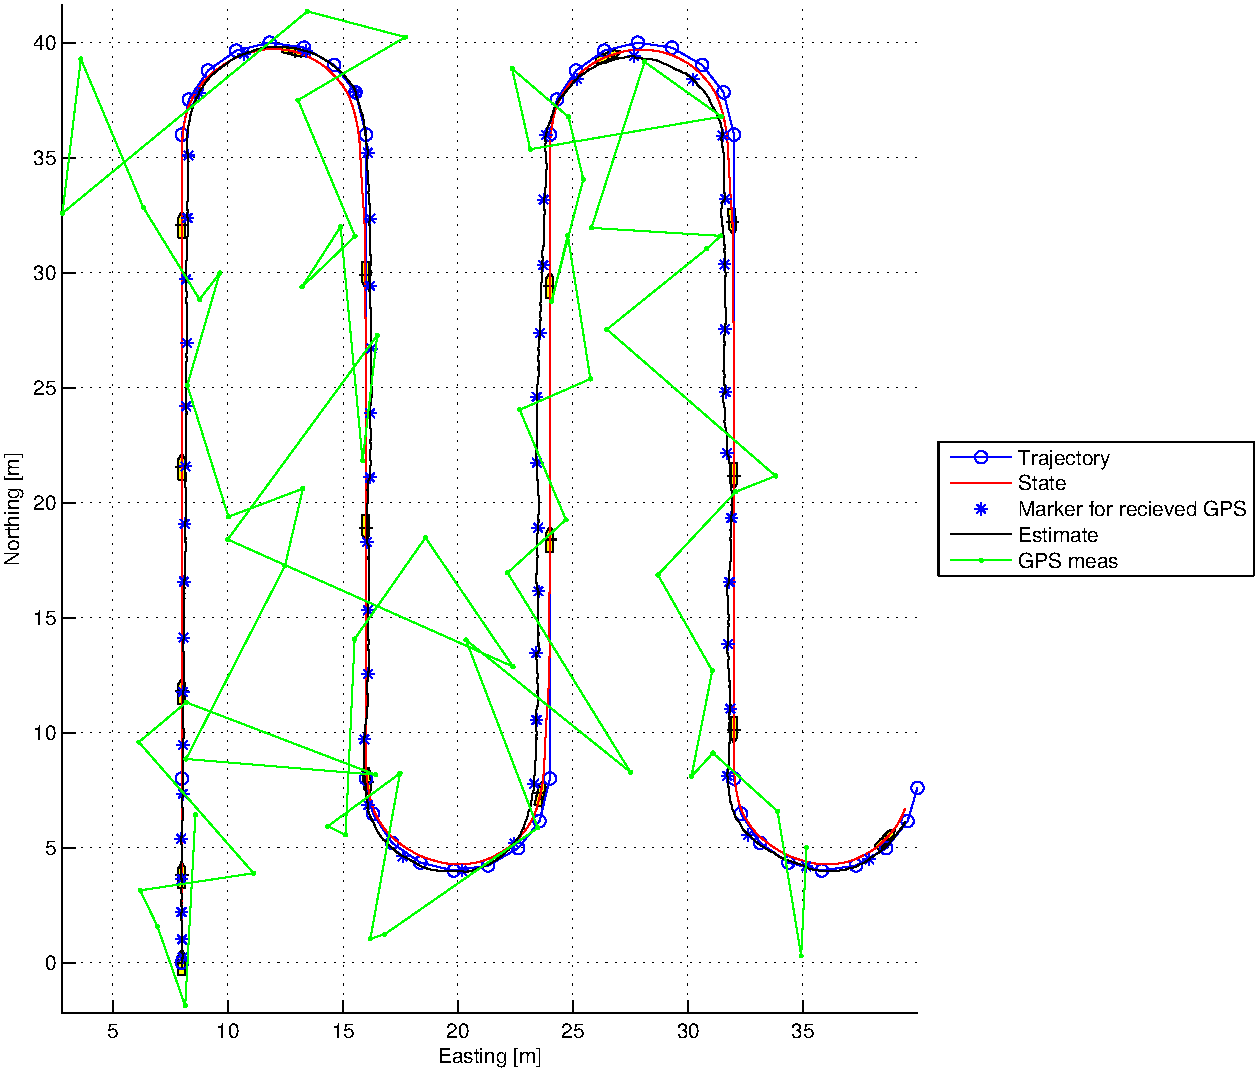
\includegraphics[width=0.48\textwidth]{../code/matlab/q0,0001}
% \caption{Simulation}
% \end{center}
% \end{wrapfigure}
As for now shows the simulation that the model of the AAUSHIP are able to follow a predetermined trajectory with a mean error of 32cm and a maximum error of 87cm. This is within the accepted limit when looking at the area of interest. When then AAUSHIPs needs to sail in formation, and cover rather large areas, then is the accuracy not very important, at least not such small derivations.

As the very end result of the project it is expected to be a complete map of the seabed at Aalborg Harbour, and a comparison with data measured from The Port of Aalborg to verify the findings of the AAUSHIP. This map needs to be measured of two or three autonomous vessels that sails in a determined formation that has not yet been decided. The formation task needs to be chosen from the location such that the formation is optimised to the specific location of interest.
 
\paragraph{Conclusion}
For now the goals are reached with a model of the AAUSHIP that can track the given trajectory. From now on is the goal to make the AAUSHIP sail in real life which is almost accomplished. Afterwards should control paradigms within formation control be tested and implemented on the AAUSHIP and the rest of the fleet. As the complete conclusion should the tests be performed in the same location of interest as the data have been taken by The Port of Aalborg. The conclusion should by that time be that the fleet can do it as good as the manual scanning performed by The Port of Aalborg.



\end{document}

%Here's a suggestion as to what an extended abstract should contain:
%
%    Background - A little history about who's done what and how your work fits in with it.
%    Aim - What you're trying to tell the audience that they don't already know (e.g. Your story.)
%    Method - Why the audience should believe that the results you've got aren't made up or flawed
%    Results - Evidence that you've come up with that confirms your story
%    Conclusion - Recap of your story and its implications
%    Limitations - Why someone might doubt your story and what you've done to get rid of as much doubt as possible.
%
%What if I'm presenting a review of my progress to date and I have no original research?
%Method = literature survey.
%Results = what you've read.
